% Copyright 2007 by Till Tantau
%
% This file may be distributed and/or modified
%
% 1. under the LaTeX Project Public License and/or
% 2. under the GNU Public License.
%
% See the file doc/licenses/LICENSE for more details.

\documentclass[portuguese,10pt,xcolor=table]{bredelebeamer}
\setbeameroption{show notes}

\usepackage[brazil]{babel}
\usepackage[utf8]{inputenc}
\usepackage{times}
\usepackage{varwidth}
\usepackage{listings} % Código de programas
\usepackage{tikz}
\usepackage[tikz]{bclogo}
\usepackage{tikzsymbols}
\usepackage{pifont}
\usepackage{array}
\usetikzlibrary{arrows,shapes}

\usetikzlibrary{calc,decorations.pathmorphing,patterns}
\pgfdeclaredecoration{penciline}{initial}{
	\state{initial}[width=+\pgfdecoratedinputsegmentremainingdistance,
auto corner on length=1mm,]{
	\pgfpathcurveto%
{% From
	\pgfqpoint{\pgfdecoratedinputsegmentremainingdistance}
{\pgfdecorationsegmentamplitude}
}
{%  Control 1
	\pgfmathrand
\pgfpointadd{\pgfqpoint{\pgfdecoratedinputsegmentremainingdistance}{0pt}}
{\pgfqpoint{-\pgfdecorationsegmentaspect
\pgfdecoratedinputsegmentremainingdistance}%
{\pgfmathresult\pgfdecorationsegmentamplitude}
}
}
{%TO 
	\pgfpointadd{\pgfpointdecoratedinputsegmentlast}{\pgfpoint{1pt}{1pt}}
}
}
\state{final}{}
}



\everymath{\displaystyle}
\tikzstyle{every picture}+=[remember picture,decoration=penciline]
\DeclareTextFontCommand{\textdf}{\bfseries\color{blue!80}}
%\tikzstyle{every node}+=[decorate]
%\tikzstyle{every path}+=[decorate]
%\tikzstyle{na} = [baseline=-.5ex]

\usepackage[T1]{fontenc}

\def\lecturename{IMD0012 - Introdução às técnicas de programação}

\title{\insertlecture}

\author{Prof. Fernando Figueira\\(adaptado do material do Prof. Rafael Beserra Gomes)}

\institute{UFRN}

\subject{Strings}

\lecture[]{Strings}{}

\date{}

\def\exe[#1]{\color{gray}#1\color{black}}
\def\exp[#1]{\color{gray}<\textit{#1}>\color{black}}
\def\espaco{\color{gray}\hspace{0.1cm}\color{black}}
\def\espaco{\color{blue}␣\color{black}}
\def\inativo[#1]{\color{gray}#1\color{black}}

\definecolor{deepgreen}{rgb}{0,0.5,0}
\lstset{
	language=C,
basicstyle=\footnotesize\ttfamily,
%basicstyle=\scriptsize\ttfamily,
keywordstyle=\footnotesize\bfseries\sffamily,
%keywordstyle=\scriptsize\bfseries\sffamily,
showstringspaces=false,
numbers=left,
numberstyle=\footnotesize,
stepnumber=1,
numbersep=5pt,
tabsize=4,
%backgroundcolor=\color{blue!05},
backgroundcolor=\color{gray!35},
showspaces=false,
showtabs=false,
stringstyle=\ttfamily\color{red!80!brown},
commentstyle=\ttfamily\color{blue!80},
keywordstyle=\bfseries\color{deepgreen},
escapeinside={\%*}{*)}
}
\renewcommand{\lstlistingname}{Código}
\begin{document}

\usebackgroundtemplate{%
	
\includegraphics[width=\paperwidth,height=\paperheight]{background2}
}
\begin{frame}
	\maketitle
	\begin{center}
		\tiny
		Material compilado em \today.\\
		Licença desta apresentação:\\
		
\includegraphics[height=1.0cm]{by-nc-nd.png}\\
		http://creativecommons.org/licenses/
	\end{center}
\end{frame}


\def\GN[#1]{\colorbox{gray!40}{#1}}
\def\RN[#1]{\colorbox{red!40}{#1}}
\def\BN[#1]{\colorbox{blue!40}{#1}}
\def\ON[#1]{\colorbox{orange!40}{#1}}
\def\WN[#1]{\colorbox{white!40}{#1}}


	\section{Strings em C}

		\begin{frame}[c]
			\begin{center}
				\structure{\large \insertsection }
			\end{center}
		\end{frame} 

		\begin{frame}{\insertsection} 
			\begin{itemize}
				\item \textdf{Strings}: conceito abstrato de uma sequência de caracteres
				\item Representação em C: vetor de caracteres ou literais (entre aspas duplas)
			\lstinputlisting{vetorLiteral.c}
				\item caractere '\textbackslash0' indica o final da string, é adicionado automaticamente na string literal
			\end{itemize}
		\end{frame}

		\begin{frame}{Representação da String na memória}
			Exemplo de dados na memória:
			\tiny
			\setlength{\tabcolsep}{0pt}	
			\begin{table}
				\begin{tabular}{|@{\hskip 0.1cm}c@{\hskip 0.1cm}|c|c|c|c|c|c|c|c|c|c|@{\hskip 0.1cm}c@{\hskip 0.1cm}|}
					\hline
					\textbf{Endereço} & & & & & & & & & \textbf{valor} & \textbf{tipo} & \textbf{identificação}\\\hline
					0xbffff22c & \GN[0]&\GN[0]&\GN[0]&\GN[0]&\GN[0]&\GN[1]&\GN[0]&\GN[1]& 5 & \textbf{inteiro curto} & valorIndice\\\hline
					0xbffff22d & \BN[0]&\BN[1]&\BN[0]&\BN[0]&\BN[0]&\BN[0]&\BN[1]&\BN[0]& 'B' & \textbf{caractere} & letra1\\\hline
					0xbffff22e & \BN[0]&\BN[1]&\BN[0]&\BN[0]&\BN[0]&\BN[0]&\BN[1]&\BN[1]& 'C' & \textbf{caractere} & letra2\\\hline
					0xbffff22f & \RN[1]&\RN[1]&\RN[0]&\RN[1]&\RN[1]&\RN[1]&\RN[0]&\RN[1]& 4.6 & \textbf{real} & precoGasolina\\\hline
					0xbffff230 & \RN[1]&\RN[1]&\RN[0]&\RN[0]&\RN[1]&\RN[1]&\RN[0]&\RN[0]& & & \\\hline
					0xbffff231 & \RN[0]&\RN[1]&\RN[0]&\RN[0]&\RN[1]&\RN[1]&\RN[0]&\RN[0]& & & \\\hline
					0xbffff232 & \RN[0]&\RN[1]&\RN[0]&\RN[0]&\RN[0]&\RN[0]&\RN[0]&\RN[0]& & & \\\hline
					0xbffff233 & \BN[0]&\BN[1]&\BN[0]&\BN[0]&\BN[1]&\BN[0]&\BN[0]&\BN[1]& 'I' & \textbf{caractere} & palavra[0]\\\hline
					0xbffff234 & \BN[0]&\BN[1]&\BN[0]&\BN[0]&\BN[1]&\BN[1]&\BN[0]&\BN[1]& 'M' & \textbf{caractere} & palavra[1]\\\hline
					0xbffff235 & \BN[0]&\BN[1]&\BN[0]&\BN[0]&\BN[0]&\BN[1]&\BN[0]&\BN[0]& 'D' & \textbf{caractere} & palavra[2]\\\hline
					0xbffff236 & \BN[0]&\BN[0]&\BN[0]&\BN[0]&\BN[0]&\BN[0]&\BN[0]&\BN[0]& '\textbackslash 0' & \textbf{caractere} & palavra[3]\\\hline
					0xbffff237 & \BN[0]&\BN[1]&\BN[1]&\BN[0]&\BN[0]&\BN[1]&\BN[1]&\BN[0]& 'f' & \textbf{caractere} & palavra[4]\\\hline
					0xbffff238 & \GN[0]&\GN[0]&\GN[0]&\GN[0]&\GN[0]&\GN[1]&\GN[0]&\GN[1]& 5 & \textbf{inteiro curto} & valorIndice\\\hline
				\end{tabular}
			\end{table}
			\normalsize
		\end{frame}
		
		\begin{frame} 
			Declaração e inicialização:
			\lstinputlisting{string2.c}
			Depois da declaração, atribuições devem ser caractere a caractere
		\end{frame}

		\begin{frame} 
			Equivalência char $\leftrightarrow$ int:\\

			\textbf{Maiúsculas:}\\
			$'A' \leftrightarrow 65$\\
			$'B' \leftrightarrow 66$\\
			$'C' \leftrightarrow 67$\\
			\vdots
			$'Z' \leftrightarrow 90$\\
		
			\textbf{Minúsculas:}\\
			$'a' \leftrightarrow 97$\\
			$'b' \leftrightarrow 98$\\
			$'c' \leftrightarrow 99$\\
			\vdots
			$'z' \leftrightarrow 122$\\
			
		\end{frame}

		\begin{frame} 
			Consulte \textbf{man ascii}\\
		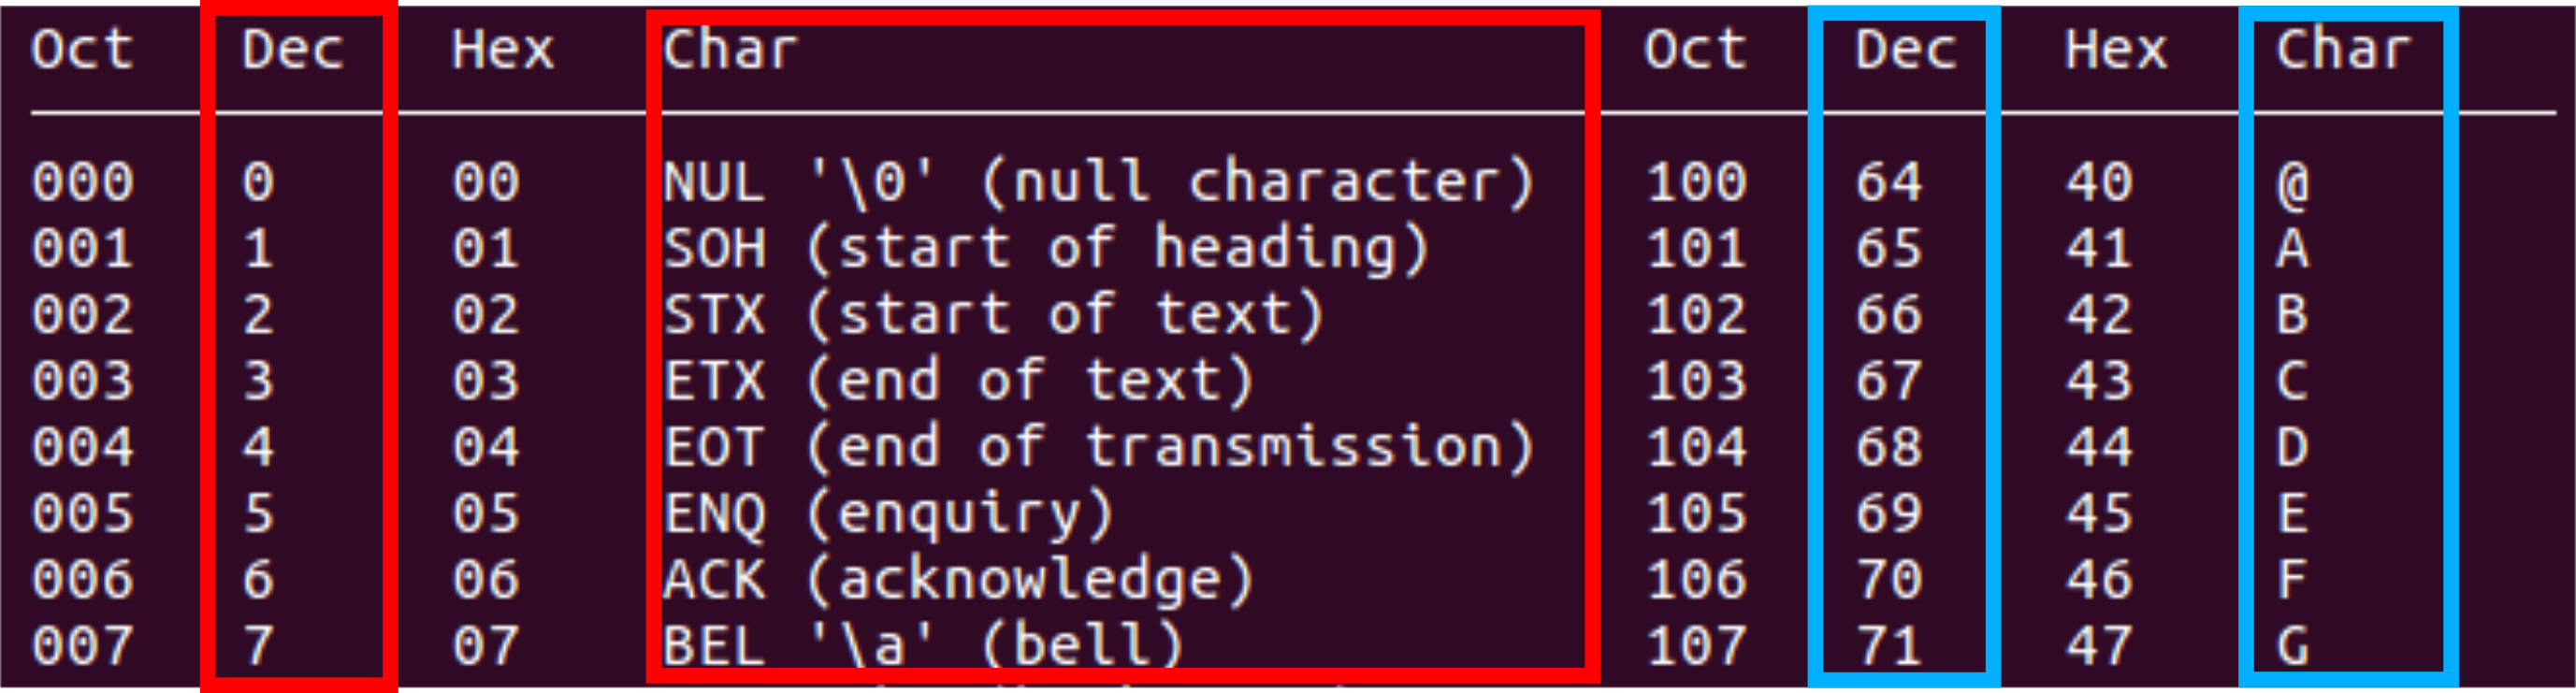
\includegraphics[height=3.0cm]{ascii.png}
		\end{frame}

		\begin{frame} 
			Equivalência char $\leftrightarrow$ int:\\

			$'s' \leftrightarrow 115$\\
			$'t' \leftrightarrow 116$\\
			$'o' \leftrightarrow 111$\\
			\lstinputlisting{ascii.c}
		\end{frame}

	\section{Escrita de strings na tela}

		\begin{frame}[c]
			\begin{center}
				\structure{\large \insertsection}
			\end{center}
		\end{frame} 

		\begin{frame}{\insertsection} 
			Ao contrário de outros tipos, um \textdf{vetor de char} pode ser escrito no printf!
			\begin{itemize}
				\item use \%s no especificador de formato, a escrita é feita até o caractere nulo ('\textbackslash0')
					\lstinputlisting{printf1.c}
			\end{itemize}
		\end{frame}


		\def\WN[#1]{\cellcolor{white!40}#1}
		\def\VN[#1]{\cellcolor{blue!40}#1}
		\def\UN[#1]{\cellcolor{green!40}#1}
		\def\RN[#1]{\cellcolor{red!40}#1}

	\section{Leitura de strings}

		\begin{frame}[c]
			\begin{center}
				\structure{\large \insertsection}
			\end{center}
		\end{frame} 

		\begin{frame} 
				\lstinputlisting{scanf.c}
			\begin{itemize}
				\item scanf
					\begin{itemize}
						\item pode ocorrer \textdf{buffer overflow}
						\item interrompe leitura no \textdf{enter ou espaço}
					\end{itemize}
				\item gets
					\begin{itemize}
						%\item consome o \textbackslash n, substituindo-o pelo \textbackslash 0
						\item pode ocorrer \textdf{buffer overflow}
						\item interrompe leitura no \textdf{enter}
					\end{itemize}
				\item fgets
					\begin{itemize}
						\item lê no máximo o segundo argumento - 1 caracteres da entrada (evita \textdf{buffer overflow})
						\item armazena o \textbackslash n na string (caso caiba!)
						\item interrompe leitura no \textdf{enter}
					\end{itemize}
			\end{itemize}
		\end{frame}

		\begin{frame} 
			Na disciplina:
			\begin{itemize}
				\item \textdf{palavra(x)}: string sem espaços com até x caracteres $\rightarrow$ \textdf{scanf}
				\item \textdf{frase(x)}: string com espaços com até x caracteres $\rightarrow$ \textdf{gets}
				\item o gcc emite um warning sobre \textdf{buffer overflow} ao usar \textdf{gets}
				\item os casos de testes obedecem aos limites estabelecidos
			\end{itemize}
		\end{frame}



	\section{Percorrendo uma string}
		\begin{frame}[c]
			\begin{center}
				\structure{\large \insertsection}
			\end{center}
		\end{frame} 

		\begin{frame}{\insertsection} 
			\begin{itemize}
				\item A função strlen (de string.h) retorna a quantidade de caracteres
				\item Ex: ler uma frase(100) e trocar todos os espaços por -
					\lstinputlisting{processaString1.c}
			\end{itemize}
		\end{frame}



		\begin{frame}
			\begin{alertblock}{\ding{46} Exercício em sala}
				Uma das regras mais conhecidas da ortografia no português é que 'n' não deve preceder 'p' e 'b'. Escreva um programa que leia uma frase(20) e realize o conserto de acordo com essa regra. Por exemplo, a string ``inpedido no canto do canpo'' é transformada em ``impedido no canto do campo''.
			\end{alertblock}
		\end{frame}


		\begin{frame}
			\begin{alertblock}{\ding{46} Exercício em sala}
				Escreva um programa para ler uma frase(100) e, em seguida, escrever a mesma string em caixa alta.
			\end{alertblock}
		\end{frame}

	\section{Funções para Strings em C}

		\begin{frame}[c]
			\begin{center}
				\structure{\large \insertsection}
				\\Principais funções da biblioteca string.h
			\end{center}
		\end{frame} 
		
		\begin{frame}[c]
			strlen\\
			\lstinputlisting{strlen.c}
		\end{frame}

		\begin{frame}[c]
			strcpy\\
			\lstinputlisting{strcpy.c}
		\end{frame}

		\begin{frame}[c]
			strncpy\\
			\lstinputlisting{strncpy.c}
		\end{frame}

		\begin{frame}[c]
			strcmp\\
			\lstinputlisting{strcmp.c}
		\end{frame}



\end{document}

